\cotefile{134-2}
\scanpage{162}
\mspage{17}
\unsure{stant|stante} -- $\pi_1^{\unsure{ar|or}}(J)\simeq H^0(k,J)\bigr]$ sous une forme cohomologique, en énonçant que l'on a
\[
\Delta_0\,\mathbb{R}\Gamma_k(J^*)\simeq\mathbb{R}\Gamma_{\unsure{h|k}}(\Delta J^*[1])
\]
où $\Delta$ est la dualité de Serre, $\Delta_0$ la dualité de \unsure{Pontrjagin|Pontryagin} des groupes abéliens top. totalement disconnexes (dualité à valeurs dans $\unsure{Q|\mathbb Q}/\unsure{Z|\mathbb Z}$) $J^*$ un complexe de ind-pro-groupes algébriques sur $k$. Tenant compte de cette ``formule de dualité de Lang'' et appliquant $\mathbb{R}\Gamma_k$ à la formule de dualité \inserted{des corps de classes} géométrique, on trouve la ``formule de dualité du corps de classes arithmétique''
\[
\boxed{\Delta_0\bigl(H_!(X,F)\simeq H^*\bigl(X,D(F)[3]\bigr)}
\]
(isom de groupes topologiques tot. discontinus).

Autre remarque : lorsque $F$ n'est pas un ``faisceau étale'', mais a une structure continue comme $\alpha_p$, il faut faire attention dans la définition de $Rf_!(F)$, pour $X$ non complète, à partir de la compactifiée \inserted{$\widetilde X$} ; ainsi, si $F$ provient d'un faisceau \inserted{``admissible''} $\widetilde F$ sur $\widetilde X$, il faut avoir un triangle exact
\diagram{\begin{tikzcd}[ampersand replacement=\&,column sep=small,row sep=small]
\& Rf_!(\widehat{\widetilde F}) \arrow[dl] \& \\
Rf_!(F) \arrow[rr,dash,"{\unsure{\mid|>}}"{pos=1,anchor=center,inner sep=0pt}] \& \& R\widetilde f_*(\widetilde F)\,, \arrow[ul]
\end{tikzcd}}
% archive sheet number: 162
\scanpage{163}
\mspage{18}
où $\widehat{\widetilde F}$ est le \uline{complété formel} de $\widetilde F$ le long de $\widetilde X-X$ (nb fini de points\ldots). C'est ici, sauf erreur, que \unsure{s'amorce|s'annonce} le lien avec le corps de classes local, version cohomologique, dont je vais dire quelques mots maintenant.

E) \uline{Corps de classes local} comme formule de dualité.

Soit $V$ un anneau de val. discrète complet, à corps résiduel $k$ -- on suppose ou bien $k$ relevé en $k\subset V$ (\unsure{donc} $V\simeq\unsure{h|k}[[T]]$) ou bien $k$ parfait. Pour fixer les idées et être sur un terrain solide, je prends \inserted{d'abord} sur $K={}$corps des fractions de $V$ des coefficients \uline{finis} $F$ (comme sur $X$ tout à l'heure), et je m'intéresse aux $H^i(K,F)$ ou encore à $R\Gamma_K(F)$. L'essentiel du travail à faire consiste à définir une catégorie de coeff. convenable sur $k$ (sans doute la $\overline{\mathrm m}$ que dans D)) et un foncteur
\[
 F\longmapsto\mathbb{R}\underline{\Gamma}_K(F)\unsure{:|.}
\]
vers ces coefficients, de telle façon que l'on ait
\[
 R\Gamma_K(F)\simeq R\Gamma_h\bigl(R\underline{\Gamma}_K(F)\bigr).
\]
% archive sheet number: 163
\scanpage{164}
\mspage{19}
Ceci correspond à l'intuition (sortant immédiatement des exemples élémentaires), moyennant quoi, pour $\unsure{h|k}$ alg clos disons, les $H^0(K,F), H^1(K,F)\ldots$ ont une structure de groupes algébriques (ind-pro \ldots) sur $k$. Dans cette construction, le \unsure{schéma|schème} en anneaux sur $k$ défini par $V$ (introduit par Serre) et le ``foncteur de Greenberg'' (associant à un schéma sur $V$ un proschéma sur $k$) joueront un rôle essentiel.

Ceci posé, la formule de dualité \unsure{s'écrira|s'écrive} formellement comme dans (D) ci-dessus
\[
 \Delta R\underline{\Gamma}_K(F)\simeq R\underline{\Gamma}_K(DF[1])
\]
où $D$ est la dualité de Cartier, $\Delta$ est la dualité de Serre. Pour un corps résiduel fini, elle devient (via ``l'astuce de Lang'' plus haut)
\[
 \begin{aligned}
 \overset{\unsure{\sim}}{\Delta}_0 R\Gamma_K(F)\simeq R\Gamma_K(DF[\deleted{\unsure{1}}2]),&\quad \Delta_0\ \text{dualité de}\\
 &\quad\text{\unsure{Pontrjagin|Pontryagin}.}
 \end{aligned}
\]
Elle contient encore le corps de classes local géométrique à la Serre, et le corps de classes local arithmétique\unsure{.} sous sa forme classique.

\uline{Remarques} \unsure{a|$\alpha$}) Si $F$ est premier à la car. résiduelle, la formule est très facile et bien connue. On peut la considérer comme un cas très particulier
% archive sheet number: 164
\scanpage{165}
\mspage{20}
de la ``formule d'induction'', pour un morphisme $i:s\unsure{\relbar\joinrel\dashv|\longrightarrow}S$, en \deleted{\unsure{formule|formel}}formalisme de dualité :
\[
 i^!(D_S\unsure{P|F})=D_s(i^*(F))
\]
(on prend ici l'inclusion de $s=\operatorname{Spec}k$ dans $S=\operatorname{Spec}V$). Donc le travail à faire concerne les coefficients $p$-primaires, $p=\operatorname{car}\unsure{h|k}>0$. Le cas le plus subtil est celui d'inégales caractéristiques.

b) Le foncteur $R\underline{\Gamma}$ s'obtient en composant $Rj_*$ (où $j:U=\operatorname{Spec}K\mathrel{\relbar\joinrel\dashv}\operatorname{Spec}V=S$ est l'inclusion), avec une sorte de ``foncteur de Greenberg'', version cohomologique.

c) Dans (D) et (E), je me suis \unsure{borné|borner} à parler des coefficients \uline{finis} $F$ -- c'est pour ceux-là que je suis sûr de mon fait. Mais il est certainement vrai que la formule de dualité est encore plus riche, qu'on peut encore énoncer quelque chose \inserted{p.ex} pour \unsure{.} $F$ un schéma en groupes pas néc. fini, p.ex. un schéma abélien \inserted{(avec quelques fibres dégénérées dans (D) ?)} -- mais je n'ai jamais tiré cette question entièrement au clair, même \unsure{heuristiquement}. J'ai une vague souvenance d'un genre de formule
% archive sheet number: 165
\scanpage{166}
\mspage{21}
qui devrait être contenue dans le formalisme, savoir (si $\unsure{k|h}$ alg clos disons) : \unsure{di|de|si} $F$ schéma abélien sur $K$, $F'$ le schéma abélien dual, et $G'$ le groupe proalgébrique sur $k$ attaché ``à la Greenberg'' à son modèle de Néron, on a
\[
 H^1(K,F)\overset{?}{\simeq}\operatorname{Ext}^{1}_{k\text{-}\unsure{\mathrm{gr}|\mathrm{gr.}|\mathrm{grp}}}(G',\unsure{Q|\mathbb Q}/\mathbb Z)
\]
(NB sans aucune garantie). En principe, la
% margin note written sideways
{\reversemarginpar\margin{\unsure{conj|conj.} \unsure{mentionnée} sur les modèles de Néron devrait sortir de la machine de dualité locale\par\noindent\tikz{\draw (0,.15) .. controls (.20,.15) and (.28,.10) .. (.32,-.04) .. controls (.32,.09) and (.43,.12) .. (.91,.12);}}}

d) Tu pourrais demander à Deligne s'il n'a pas approfondi les questions (D) et (E) dernièrement.

\figure{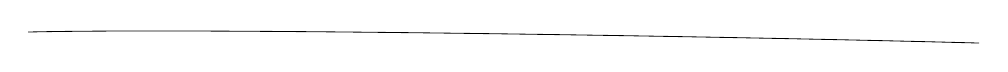
\begin{tikzpicture}[x=\linewidth,y=1cm]
\draw[line width=.3pt] (0,0) .. controls (.18,.05) and (.72,-.05) .. (.996,-.14);
\end{tikzpicture}}

(F) \uline{Portée et limites de la topologie} fppf

Depuis les essais de Serre de trouver une ``coh. de Weil'' en utilisant la cohomologie d'un schéma à coefficients non seulement discrets $\mathbb Z/p^n\mathbb Z$ ($n\unsure{\mapstochar\relbar\joinrel\dashv|\longrightarrow}\infty$), ou $\mu_{p^n}$ ($n\mathrel{\mapstochar\relbar\joinrel\dashv}\infty$), mais aussi continus (\inserted{p.ex} $W_n$, $n\unsure{\relbar\joinrel\dashv|\longrightarrow}\infty$), qui donnait de bons résultats pour récupérer un $H^1$ correct, pendant de nombreuses années j'étais \inserted{resté} sur l'impression, que j'essayais en vain de préciser, qu'une ``coh. de Weil'' ``$p$-adique''\unsure{:} correcte, en car. $p>0$, devait pouvoir sortir d'une façon ou d'une autre de la cohomologie fppf, pour des coefficients finis p.ex., ou des coefficients
% archive sheet number: 166
\scanpage{167}
\mspage{22}
plus généraux, groupes algébriques sur $\unsure{k|h}$. La construction en (B) de complexes de \unsure{jacobiennes|jacobienne} locales était, évidemment, \inserted{un peu} \unsure{lié|liée} à cet espoir -- l'homologie donnerait peut-être ce que la cohomologie nous cèle ! Depuis lors, on dispose du formalisme de la cohomologie cristalline, et on sait \inserted{(Berthelot)} que (du moins \deleted{que} pour $X$ projectif et lisse) elle a les propriétés correctes. Si on l'utilise comme une sorte d'étalon sûr à quoi ``mesurer'' les autres cohomologies, on trouve ceci : la partie de la cohomologie \unsure{cristalline} $H^i_{\mathrm{cris}}(X)$ qui peut être décrite en termes de cohomologie fppf de $X$ à coefficients dans des $k$-groupes algébriques, n'est qu'une \deleted{\unsure{faible|facile}} petite partie du $H^i$ ; de façon précise, utilisant la structure \inserted{très rigide} supplémentaire de $H^i$ (module de t.f. sur \unsure{les' anneau|l'anneau} $W(k)$ des vecteurs de Witt) provenant de l'existence de l'\unsure{hom|hom.} de Frobenius $H^i\mathrel{\mathop{\unsure{\tikz[baseline=-.4ex]{\draw (0,0)--(.53,0)--(.55,.025)--(.57,-.01);}|\longrightarrow}}\limits^{F}}H^i$ (semi-linéaire) on \unsure{trouve :|trouve} que l'on \unsure{reste|rentre} toujours dans la partie ``de pente $\leq 1$'' (alors que les pentes possibles varient entre $0$ et $i$\ldots) \unsure{Ca|Ça|Ce} explique pourquoi pour $i=1$
% archive sheet number: 167
\scanpage{168}
\mspage{23}
on a pu obtenir via fppf un $H^1$ correct, alors que pour le $H^2$ déjà tous les essais \unsure{ont|nt} été infructueux.

À vrai dire, on conjecture que \uline{toute} la partie de pente $\leq 1$ du $H^i_{\mathrm{cris}}$ provient de fppf\unsure{:|.} Mais j'ai perdu complètement contact avec ces questions -- des gens comme Mazur, Katz, Messing -- et bien sûr, Deligne -- devraient être au courant du point où en est la question.

\figure{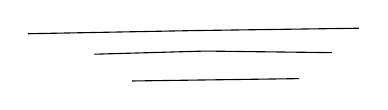
\begin{tikzpicture}[x=1cm,y=1cm]
\draw (0,0) -- (2.1,.04) -- (4.2,.07);
\draw (.84,-.26) -- (2.25,-.22) -- (3.86,-.24);
\draw (1.32,-.60) -- (3.44,-.57);
\end{tikzpicture}}

Ta question $7^{\circ}$ semble indiquer qu'il y a malentendu en ton esprit sur la signification du ``type d'homotopie'' de $X$, $X$ un topos (p.ex. le topos \unsure{étale|étal} d'un \unsure{schéma|schema}). Sans doute tu dois confondre l'\unsure{algèbre|algebre} homotopique qu'on peut faire sur $X$ à coups de faisceaux semi-simpliciaux, de champs en \unsure{tous|tout} genre, et des relations entre ceux-ci -- et cet autre point de vue où $X$ (avec sa structure si riche de topos) \unsure{disparait|disparaît} virtuellement,
% archive sheet number: 168
\scanpage{169}
\mspage{24}
pour ne devenir plus qu'un pâle élément d'une ``catégorie homotopique'' (ou \unsure{pro-homotopique|prohomotopique}), déduite de celle des topos par un processus de localisation à \unsure{brin|bras|brins} de zinc -- à première vue, tout ce qui reste encore à ce pauvre $X$, ce sont ses $\pi_i$ -- et ses groupes de \unsure{cohomologies|cohomologie} à \unsure{coefficient|coefficients} constants -- ou à la rigueur constant tordus. Quand on fouille un peu plus dans cette direction ``que reste-t-il encore à ce pauvre $X$'' on tombe précisément sur les \inserted{$n$-}champs \uline{loc.} \uline{constants} (car un $X\mathrel{\unsure{\tikz[baseline=-.5ex]{\draw (0,0)--(.52,0); \node[anchor=base,inner sep=0pt] at (.42,-.08) {$f$};}|\overset{f}{\longrightarrow}}}X'$ qui est une équivalence d'homotopie induit une $(n+1)$-équivalence entre les cat. de $n$-champs loc. \unsure{constant|constants} sur $X$ et sur $X'$) -- qui contiennent bien sûr les complexes \inserted{de \unsure{chaines|chaînes}} abéliens \inserted{de long. $n$} à faisceaux de coh. loc. constants, et l'hypercohomologie de ceux-ci. C'est ainsi qu'on arrive à \deleted{\unsure{la notion|la notion du}} \inserted{ce} triangle de \inserted{\uline{\unsure{\textquoteleft|``}Objets\unsure{\textquoteright|''|{}}}} se déterminant mutuellement
\diagram{\begin{tikzcd}[ampersand replacement=\&,column sep=-1.25em,row sep=large]
\& \begin{gathered}
\text{topos (ou espace top., ou}\\
\text{ens. }{}^{1}\!/\!{}_{2}\,\text{\unsure{simpl|simpl.}) }\text{\uuline{\unsure{modulo|modúlo}}}\\
n\text{-}\text{\uline{homotopie}}
\end{gathered} \arrow[dl,leftrightarrow] \arrow[dr,leftrightarrow] \& \\
\begin{gathered}
n\text{-groupoïdes}\\
\text{(à }n\text{-équiv. \unsure{pr.|p.|près})}
\end{gathered} \arrow[rr,leftrightarrow] \& \& \begin{gathered}
n\text{-catégories ``spéciales'' (à}\\
n\text{\unsure{..|-}équivalence près)}
\end{gathered}
\end{tikzcd}}
% archive sheet number: 169
